\documentclass[computers,article,submit,pdftex,moreauthors]{Definitions/mdpi} 

%=================================================================
% MDPI internal commands - do not modify
\firstpage{1} 
\makeatletter 
\setcounter{page}{\@firstpage} 
\makeatother
\pubvolume{1}
\issuenum{1}
\articlenumber{0}
\pubyear{2026}
\copyrightyear{2026}
%\externaleditor{Firstname Lastname} % More than 1 editor, please add `` and '' before the last editor name
\datereceived{ } 
\daterevised{ } % Comment out if no revised date
\dateaccepted{ } 
\datepublished{ } 
%\datecorrected{} % For corrected papers: "Corrected: XXX" date in the original paper.
%\dateretracted{} % For retracted papers: "Retracted: XXX" date in the original paper.
%\doinum{} % Used for some special journals, like molbank
%\pdfoutput=1 % Uncommented for upload to arXiv.org
%\CorrStatement{yes}  % For updates
%\longauthorlist{yes} % For many authors that exceed the left citation part
%\IsAssociation{yes} % For association journals

%=================================================================
% Add packages and commands here. The following packages are loaded in our class file: fontenc, inputenc, calc, indentfirst, fancyhdr, graphicx, epstopdf, lastpage, ifthen, float, amsmath, amssymb, lineno, setspace, enumitem, mathpazo, booktabs, titlesec, etoolbox, tabto, xcolor, colortbl, soul, multirow, microtype, tikz, totcount, changepage, attrib, upgreek, array, tabularx, pbox, ragged2e, tocloft, marginnote, marginfix, enotez, amsthm, natbib, hyperref, cleveref, scrextend, url, geometry, newfloat, caption, draftwatermark, seqsplit
% cleveref: load \crefname definitions after \begin{document}


\usepackage{pgfplots}
\pgfplotsset{compat=1.18}
\usepackage{listings}
\lstset{basicstyle=\ttfamily\small, columns=fullflexible, frame=single}


%=================================================================
% Please use the following mathematics environments: Theorem, Lemma, Corollary, Proposition, Characterization, Property, Problem, Example, ExamplesandDefinitions, Hypothesis, Remark, Definition, Notation, Assumption
%% For proofs, please use the proof environment (the amsthm package is loaded by the MDPI class).

%=================================================================
% Full title of the paper (Capitalized)
\Title{Towards LLM-as-a-Judge for Parser Error Clarity: A Controlled Baseline Study with Obfuscated Inputs}

% Author Orchid ID: enter ID or remove command
\newcommand{\orcidauthorA}{0000-0002-7171-7979} % Add \orcidA{} behind the author's name
%\newcommand{\orcidauthorB}{0000-0000-0000-000X} % Add \orcidB{} behind the author's name

% Authors, for the paper (add full first names)
\Author{Ki Yung Ahn $^{1}$\orcidA{}, Firstname Lastname $^{2}$ and Firstname Lastname $^{2,}$*}

%\longauthorlist{yes}

% MDPI internal command: Authors, for metadata in PDF
\AuthorNames{Ki Yung Ahn, Firstname Lastname and Firstname Lastname}

% Affiliations / Addresses (Add [1] after \address if there is only one affiliation.)
\address{%
$^{1}$ \quad Affiliation 1; kya@hnu.kr\\
$^{2}$ \quad Affiliation 2; e-mail@e-mail.com}

% Contact information of the corresponding author
\corres{Correspondence: kya@hnu.kr; Tel.: (optional; include country code; if there are multiple corresponding authors, add author initials) +xx-xxxx-xxx-xxxx (K.Y.A.)}

% Current address and/or shared authorship
%\firstnote{Current address: Affiliation.}  
% Current address should not be the same as any items in the Affiliation section.

%\secondnote{These authors contributed equally to this work.}
% The commands \thirdnote{} till \eighthnote{} are available for further notes.

%\simplesumm{} % Simple summary

%\conference{} % An extended version of a conference paper

\abstract{We study the possibility of judging parser error-message clarity with LLMs despite their prior-knowledge bias that masks differences between informative and uninformative error messages. The problem matters because without controlling this bias, LLM-based evaluations over-credit parsers for more commonly used syntax even when messages are unclear. We obfuscate terminal symbols related to syntax errors and measure correction accuracy difference for the informative error message and the baseline uninformative error message, handled by several LLMs (Gemma 3 and CodeGemma variants, GPT-5.2 Instant/Thinking) under prompts pairing code snippets and their error messages. Only certain model variants (Gemma 3 12B and GPT 5.2 variants) were able to exhibit the desired clarity-driven performance differences for obfuscated inputs, indicating that input obfuscation could be a practical lever for LLM-as-judge assessments of parser diagnostics, but model selection is crucial.}

\keyword{LLM-as-a-judge; parser error messages; input obfuscation; compiler diagnostics; automated evaluation}

% The fields PACS, MSC, and JEL may be left empty or commented out if not applicable
%\PACS{J0101}
%\MSC{} %%% generated by CoPilot need to be checked ==> \MSC{68N15; 68T50; 68Q42}
%\JEL{}

\begin{document}

\section{Introduction}

It is widely accepted that top-down parsers
(LL-based, recursive descent) tend to produce
clearer error messages than bottom-up parsers
(LR-based, table-driven).  Qualitative explanation
why this is the case can be found in many college level textbooks
\cite{AhoSethiUllman2006,CooperTorczon2011,Louden1997};
errors are detected earlier and have clearer syntactic context
in top-down parsers than in bottom-up parsers.

Quantitative analysis on this aspect, however, has been limited
due to the difficulty of performing controlled studies.
Traditional approach would involve human surveys where
participants are shown code snippets with syntax errors
along with error messages produced by different parsers.
Human survey tends to be costly and time-consuming. More crucially,
it is extremely difficult to select appropriate participants
for the purpose of the study. A mixture of beginners and experts would
likely lead to noisy results. Even if we can select participants with
similar years of programming experience, there could still be bias from
the different exposure to the specific programming language syntax
and compiler implementations.

In this work, we consider an LLM-as-a-judge approach to perform
a controlled study to evaluate the clarity of error messages.
Using LLMs clearly reduces the cost and time compared to
human surveys. More importantly, we can ensure that the judge has
uniform experience on every experiment because what LLM has learned
is fixed at the time of training. However, LLMs are also biased
from the exposure to existing programming language syntax and
compiler implementations. This bias of LLMs could be
even more problematic for the evaluation than human participants,
because the tendency to ``best guess'' from the trained knowledge
often seems to dominate the behavior LLMs exhibit.
To mitigate this bias, we propose to obfuscate the inputs by
replacing the terminal symbols of the language with some other symbols,
in order to reduce the effect of prior knowledge of the LLM judge.

Our thesis is that by reducing the effect of prior knowledge,
the clarity of error messages could have more impact on
the performance of the LLM judge in fixing syntax errors.
We design and perform an experiment to show that there exists
an LLM judge where our thesis holds, for the very baseline case
of error message clarity, that is, distinguishing between
an informative error message and the worst uninformative error message.
More specifically, our experiment demonstrates that well-chosen
obfuscation could enable an LLM judge to distinguish the difference
in error message clarity, at least for the baseline case.

Our contributions are as follows:
\begin{itemize}
\item
We identify the prior-knowledge dominance problem of using
LLMs as judges for evaluating parser error message clarity,
and propose obfuscation of input code snippets to mitigate the problem.
\item
We design a controlled experiment to prove the concept
that an LLM judge can evaluate the clarity of error messages,
by comparing the performance of the LLM judge for the baseline case
of distinguishing informative and uninformative error messages.
\item
We perform the designed experiment with smaller LLM models
that could run in stand-alone local environments,
which makes our results highly reproducible
even on ordinary personal computing resources.
\item
We also performed the same experiment with GPT-5.2 models
to compare the results with larger LLM models to see the effect of
model size and advanced iterative thinking capability
on the evaluation of error message clarity.
\end{itemize}

\section{Background}
In this section, we discuss two subcategories of
the LLM-as-a-judge approach, and which one is suitable for
evaluating parser error message clarity.

\subsection{LLM-as-a-judge by the Rule Book}
The idea of using LLMs as judges \cite{zheng2023judging}
for various tasks has been gaining popularity recently,
expanding to different application areas, including UI/UX evaluation
\cite{duan2024generating,duan2024uicrit,lee2024applying}.
In a typical LLM-as-a-judge approach, the ``common sense'' of
an LLM is exploited, along with careful prompting, so that
the LLM judge is likely to produce similar results to human evaluations.
Sometimes systematic rules are provided to the LLM judge
to guide its judgement.

For example, the judging rules (or, grading policies) may be explained
through prompt to an LLM, as they are explained to human judges.
Then, the LLM judge is asked to evaluate the target artifacts
according to the explained rules.  Majority of LLM-as-a-judge approach
is based on this rule book setting.  This rule book setting, however,
is not suitable for evaluating error message clarity, because
such rules for error message clarity are not well-defined.
Top-down and bottom-up parsers are compared qualitatively with
some examples, but formal rubric for evaluation is rarely provided.

Relying on the ``common sense'' of LLMs without well-defined rules
would only likely to fulfill self-prophecy for our case.
The training data regarding parsing error messages are
likely to include standard textbooks on compilers and parsing.
Thus, if it looks like an error message from a top-down parser,
the ``common sense'' of LLMs would judge them to be clearer.
This is no more than reproducing memorized patterns from the training data.

\subsection{LLM-as-a-judge by Task Performance}
Some judgements need to be made by observing the performance of
the participants on specific tasks. For example, judging which
prompt works better for the LLM to perform a specific task is not
suitable for the rule book setting.  Instead, one needs to measure
objective metrics such as the accuracy or processing time of
the specific task performed by an LLM for different prompts.
Such idea has been explored in automated prompt optimizations
\cite{zhou2023large,fernando2023promptbreeder}.

In our case, prompt should include a code snippet and an error message,
and the task for the LLM judge would be to fix the syntax error
to output corrected code.  Then, the clarity of error messages
may be benchmarked by the rate of correctly fixed code.
If our thesis holds, that is, the clarity of error messages
could have impact on the behavior of LLM judges, we would expect
to use such LLM judges to evaluate the clarity of error messages
between different parsers.  More specifically, parsers producing
error messages that lead to higher accuracy in fixing syntax errors
for the LLM judge would be considered to provide clearer error messages.

\subsection{Setting the Baseline with Obfuscated Inputs}
When evaluating error message clarity, there is an obvious baseline for
the worst, that is, the most unclear error message, which provides
information no other than the fact that there exists an error.
For LLMs, the baseline for this evaluation is corrupted
in the sense that they can fix wide range of syntax errors
for those worst possible error messages, even for newly invented
programming language syntax. What we would like to see is that
the LLM judge performs better with informative error messages,
than the baseline case of the worst uninformative error messages.

When a human participant is asked to fix a syntax error for
a code of an unknown syntax, she would most likely ask
what programming language it is. When the human participant
notice that it is not a familiar programming language, she would
intentionally be more cautious not to rely on her knowledge of
existing programming languages familiar to her. In contrast,
unlike human participants, an LLM typically answers to the prompt
as best as it can, according to the `knowledge' obtained during training,
which includes the syntax of various existing programming languages.
The LLM would apply similar patterns for syntax errors and
their fixes commonly found in its training data, even without
any useful information from the provided error messages.
Then, it would be impossible to evaluate which error message is clearer
because the judge's behavior is indistinguishable between different error messages.

Our idea is to replace the terminal symbols, which are related to
the cause of the syntax error, with less commonly used symbols,
while keeping the grammar structure intact. For example, when
the code snippet has a syntax error for mismatched parentheses,
\verb|( | and \verb| )| may be replaced with
\verb|begin| and \verb|end|, provided that
they are not keywords of the programming language
in which the code snippet is written.
By obfuscating the terminal symbols in this way,
we expect that the LLM judge would be less likely to apply its prior knowledge
and would rely more on the information provided in the error message.

\section{Experiment Design}

The aim for our experiment is to establish baseline
for the syntax error message reporting a mismatched closing curly brace.
Consider the code snippet below.
\begin{quote}
    \verb|if (x > 0) { a = 1; } else b = 2; }|
\end{quote}
This is an imaginary programming language,
which we will call \emph{brace-lang}, with a C-like syntax
for the conditional statement.
An informative error message we provide for this code snippet is
\begin{quote}
    \verb|unexpected ']' after else clause (if statement already closed)|
\end{quote}
whereas the worst uninformative error message is simply
\begin{quote}
    \verb|syntax error|.
\end{quote}
~

For each error message quality (informative vs. uninformative),
we ask an LLM to fix the syntax error in the code snippet above,
with the prompt template shown in Figure \ref{fig:prompt-template}.
The correct fix should either
(1) remove the extraneous closing curly brace
    (\verb|}|) at the end
or
(2) add an opening curly brace (\verb|{|) after
    \verb|else| to match the closing curly brace.
That is, the intended correct output is either one of the following:
\begin{enumerate}[label=(\arabic*)]
\item \verb|if (x > 0) { a = 1; } else b = 2;| or
\item \verb|if (x > 0) { a = 1; } else { b = 2; }|.
\end{enumerate}
We do not consider ``\verb|if (x > 0) a = 1; else b = 2;|'',
removing both curly braces, as a correct fix, because the informative error message
indicates that the closing curly brace is unexpected after \verb|else|
and that \verb|if| statement is already closed.

\begin{figure}%[htbp]
\begin{quote}
\begin{lstlisting}
Fix the syntax error in the code below using ONLY the error message,
without using the pre-trained knowledge.

Error message:
{{syntax error message here}}

Code:
```
{{code snippet with syntax error here}}
```

Output ONLY the fixed code inside the triple backquote code block.
\end{lstlisting}
\end{quote}
\caption{Prompt template for asking an LLM to fix a syntax error.}
\label{fig:prompt-template}
\end{figure}

For this original language variant \emph{brace-lang},
designed to work as a control group, we expect the LLM judge
fail to distinguish the quality of error messages, because
it is likely to lean heavily on the prior knowledge of C-like syntax
to fix the syntax error even with the worst error message ``\verb|syntax error|''. 
This language variant is to act as a control group, because
the behavior of LLM judge is actually the same for both error messages
in the result of our experiment, as we will see later in this article. 

We apply two different obfuscation schemes to the code snippet above,
to create two additional language variants, namely,
\emph{bracket-lang} and \emph{gibberish-lang},
as summarized below.
In \emph{bracket-lang}, curly braces
\verb|{| and \verb|}| are replaced with
square brackets \verb|[| and \verb|]|.
In \emph{gibberish-lang}, they are replaced with
rather arbitrary symbols \verb|@| and \verb|#|.
The informative error message and the intended corrections are
also adjusted accordingly for each language variant.

\begin{table}[htbp]
\caption{Language variants used in the experiment and the intended corrections for the code snippet in each variant.}
\label{tab:language-variants}
\begin{tabular}{|l|p{5cm}|p{5cm}|}
\hline
\textbf{Language} & \textbf{Code Snippet} & \textbf{Intended Corrections} \\
\hline
\emph{brace-lang} &
\verb|if (x > 0) { a = 1; }|

\verb|else b = 2; }| &
(1) remove \verb|}| at the end ~or

(2) add \verb|{| before \verb|b = 2;|
\\
\hline
\emph{bracket-lang} &
\verb|if (x > 0) [ a = 1; ]|

\verb|else b = 2; ]| &
(1) remove \verb|]| at the end ~or

(2) add \verb|[| before \verb|b = 2;|
\\
\hline
\emph{gibberish-lang} &
\verb|if (x > 0) @ a = 1; #|

\verb|else b = 2; #| &
(1) remove \verb|#| at the end ~or

(2) add \verb|@| before \verb|b = 2;|
\\
\hline
\end{tabular}
\end{table}

\section{Experiment Execution and Results}

For each prompt, 50 trials are performed. There is one prompt for
each combination of language variant and error message quality.
That is, 100 trials for each language variant, 50 with informative
error message and 50 with the worst error message, are performed.
For each LLM model variants, total of 300 trials are performed for
the three language variants.
We note that preliminary experiments with 25 trials per condition yielded proportionally consistent results, suggesting that the 50-trial sample size is adequate to capture the clarity distinction metric reliably.

We ran experiments over several variants of
Gemma 3 \cite{gemma2025} models (4B, 12B, and 27B)
and CodeGemma \cite{codegemma2024} models (2B, 7B, and 7B-instruct)
using the Ollama \cite{ollama} framework. 

\subsection{Experiments over Gemma 3 and CodeGemma Model Variants:}
We ran experiments over several variants of
Gemma 3 models (4B, 12B, and 27B) and
CodeGemma models (2B, 7B, and 7B-instruct)
using the Ollama framework.
Among them, only Gemma 3 12B model behaved to distinguish the clarity
between the informative and uninformative error messages
for the \emph{bracket-lang} variant, as summarized below:
\begin{itemize}
\item 50/50 correct fixes for \emph{brace-lang} with the worst error message,
\item 
50/50 correct fixes for \emph{brace-lang} with the informative error message,
\item 0/50 correct fixes for \emph{bracket-lang} with the worst error message,
% (producing same output as for \emph{brace-lang}),
\item 50/50 correct fixes for \emph{bracket-lang} with the informative error message,
\item 0/50 correct fixes for \emph{gibberish-lang} with the worst error message,
\item 0/50 correct fixes for \emph{gibberish-lang} with the informative error message.
\end{itemize}
For the \emph{brace-lang} and \emph{bracket-lang} variants,
the outputs were always exactly the same for the same prompt settings
(that is, for the same language variant and same error message quality)
across 50 trials. For the \emph{gibberish-lang} variant,
there were some different outputs for the same prompt setting
across 50 trials, but none of them were correct fixes.

The other Gemma 3 models (2B and 7B) were not able to distinguish
the clarity of error messages for any language variants including
\emph{bracket-lang}. None of the CodeGemma models were able to
distinguish the clarity of error messages for the \emph{brace-lang}
variant either. They simply could not produce correct fixes.

\subsection{Experiments over GPT-5.2 Model Variants}
We also tried with GPT-5.2 Instant and Thinking
(via \url{chatgpt.com} as of early Jan 2026) with the same prompts.
In general, GPT-5.2 models produced more diverse outputs
across 50 trials for the same prompt settings,
compared to the Gemma 3 12B model.

GPT-5.2 Instant performed as follows:
\begin{itemize}
\item
% https://chatgpt.com/c/6956ae0f-7768-8323-8ddc-eaecbac59868
% https://chatgpt.com/c/6956ae60-5c44-8322-b9ef-ace41246701f
50/50 correct fixes for \emph{brace-lang} with the worst error message,
\item
50/50 correct fixes for \emph{brace-lang} with the informative error message,
\item
12/50 correct fixes for \emph{bracket-lang} with the worst error message,
\item
50/50 correct fixes for \emph{bracket-lang} with the informative error message,
\item
0/50 correct fixes for \emph{gibberish-lang} with the worst message,
\item
19/50 correct fixes for \emph{gibberish-lang} with the informative error message,
\end{itemize}
These results using GPT-5.2 Instant aligns with
our results using the Gemma 3 12B model, where
the distinction of error message clarity is most apparent
for the \emph{bracket-lang} variant. But unlike the Gemma 3 12B model,
GPT-5.2 Instant was also able to show some distinction
for the \emph{gibberish-lang} variant as well.

GPT-5.2 Thinking performed as follows:
\begin{itemize}
\item
50/50 correct fixes for \emph{brace-lang} with the worst error message,
\item
50/50 correct fixes for \emph{brace-lang} with the informative error message,
\item
21/50 correct fixes for \emph{bracket-lang} with the worst error message,
\item
36/50 correct fixes for \emph{bracket-lang} with the informative error message,
\item
0/50 correct fixes for \emph{gibberish-lang} with the worst message,
\item
27/50 correct fixes for \emph{gibberish-lang} with the informative error message,
\end{itemize}
What is interesting about the results using GPT-5.2 Thinking is that
baseline performance for the worst error message for the \emph{bracket-lang} variant
is corrupted because of thinking more about other possibilities for syntax error,
rather than quickly parroting the prior knowledge of C-like syntax, which sometimes
leads to correct fixes even with the worst error message.

For the \emph{gibberish-lang} variant, GPT-5.2 Thinking was able to produce
more correct fixes with the informative error message compared to GPT-5.2 Instant.

Note that the reproducibility of results using the GPT model
may be limited as the underlying model is likely to be
continuously fine-tuned and updated frequently,
as being current version of serviced online GPT models.

\begin{figure}[htbp]
\centering

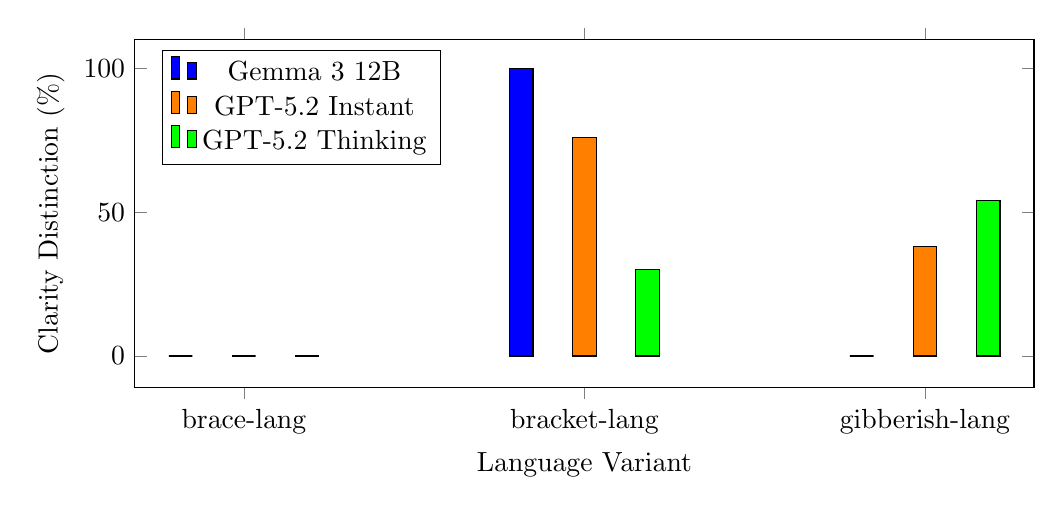
\begin{tikzpicture}
\begin{axis}[
  xlabel={Language Variant},
  ylabel={Clarity Distinction (\%)},
  ymax=110,
  width=13cm,
  height=6cm,
  xtick={1,2,3},
  xticklabels={brace-lang, bracket-lang, gibberish-lang},
  ybar,
  bar width=0.3cm,
  legend pos=north west,
]
\addplot[fill=blue] coordinates {(0.9,0) (1.9,100) (2.9,0)};
\addplot[fill=orange] coordinates {(1.0,0) (2.0,76) (3.0,38)};
\addplot[fill=green] coordinates {(1.1,0) (2.1,30) (3.1,54)};
\legend{Gemma 3 12B, GPT-5.2 Instant, GPT-5.2 Thinking}
\end{axis}
\end{tikzpicture}

\caption{Summary of the experiment results. The height of each bar
indicates the difference in correct fixes between informative
and uninformative error messages relative to the total number of trials
for each language variant. Shown are model variants that exhibited meaningful
distinction in clarity of error messages: Gemma 3 12B, GPT-5.2 Instant, and GPT-5.2 Thinking.}
\label{fig:results-summary}
\end{figure}

\subsection{Summary of Results}
To summarize the results, we devised a metric called `clarity distinction',
which is defined as the ratio of difference in number of correct fixes
between informative and uninformative error messages, relative to
the total number of trials. More specifically, the formula for calculating
clarity distinction is as follows:
\[
\text{Clarity Distinction} ~=~ \frac{C_\text{informative} - C_\text{uninformative}}{N} \times 100 ~\%
\]
where $C_\text{informative}$ and $C_\text{uninformative}$ represent
the number of correct fixes for informative and uninformative error messages,
respectively, and $N$ is the total number of trials.
The clarity distinction metrics for the models, which exhibit
meaningful distinction at least for \emph{bracket-lang},
are summarized in Figure \ref{fig:results-summary}.



\section{Experiment with Another Code Snippet}
We report another experiment we performed with a different code snippet to see
if the observed behavior in the 12B variant of Gemma 3 model is consistent.
That is, whether an obfuscated variant of the code snippet is expected to help
distinguish the clarity of error messages.
Another code snippet we used in this round of experiment is
\begin{quote}
    \verb|int x = 5 int y = 6;|
\end{quote}
The informative error message we provide for this code snippet is
\begin{quote}
    \verb|expected ';' after declaration|
\end{quote}
and the worst uninformative error message is again
\begin{quote}
    \verb|syntax error|.
\end{quote}
There is only one intended correct fix for this code snippet, which is to add
a proper delimiter, a semicolon (\verb|;|) after \verb|5| in this case.
That is, the intended correct output is:
\begin{quote}
    \verb|int x = 5; int y = 6;|
\end{quote}
We call this original language variant \emph{semi-lang}.

Missing delimiter is another common syntax error across many programming languages.
This is simpler than parenthesis-matching type of syntax errors
in our previous experiment. There could only be one intended correct fix and
the only terminal symbol related to the syntax error is the semicolon (\verb|;|).
We create two obfuscated variants of this code snippet by replacing
the semicolon with a dot (\verb|.|) or  a sharp (\verb|#|), as follows:
\begin{quote}
    \verb|int x = 5 int y = 6.|\\
    \verb|int x = 5 int y = 6#|
\end{quote}
These two language variants are called \emph{dot-lang} and \emph{sharp-lang}.
The informative error messages and the intended corrections
are also adjusted accordingly.

To our surprise, the Gemma 3 12B model could distinguish the clarity of
error messages for none of the three language variants, when run with
previous prompt template shown in Figure \ref{fig:prompt-template}.
For \emph{semi-lang}, it always produced correct fixes adding a semicolon after 5
for both error messages, showing no distinction in clarity, as we expected.
What surprised us is that it produced no correct fixes in the two obfuscated
language variants, \emph{dot-lang} and \emph{sharp-lang}, either.
Instead, the Gemma 3 12B model variant produced virtually the same output
as for \emph{semi-lang}, always adding a semicolon after 5 and also reverting
the last symbol back to semicolon about half of the time.
That is, the performance for informative error message was no better
than the baseline performance for the worst error message
in both obfuscated language variants. This indicates that
the obfuscation alone failed to mitigate the prior-knowledge dominance problem
for this code snippet with the same prompt template used previously for
parenthesis-matching type of syntax errors.

When we run the same prompts with GPT 5.2 Instant,
it failed to distinguish the clarity of error messages
for \emph{dot-lang} and \emph{sharp-lang} variants, but for opposite reasons.
GPT 5.2 Instant was able to produce correct fixes all the time regardless of
error messages in both obfuscated language variants, showing no distinction in clarity.

We were able to make Gemma 3 12B variant perform above the baseline
for \emph{dot-lang} and \emph{sharp-lang}, by modifying the prompt template
as shown in Figure \ref{fig:prompt-template-2}, emphasizing not to rely too much
on pre-trained knowledge, especially not to fall back to C-like syntax.
With this modified prompt template the Gemma 3 12B model performed as follows:
\begin{itemize}
\item
50/50 correct fixes for \emph{semi-lang} with the worst error message,
\item
50/50 correct fixes for \emph{semi-lang} with the informative error message,
\item
0/50 correct fixes for \emph{dot-lang} with the worst error message,
\item
11/50 correct fixes for \emph{dot-lang} with the informative error message.
\item
0/50 correct fixes for \emph{sharp-lang} with the worst error message,
\item
50/50 correct fixes for \emph{sharp-lang} with the informative error message.
\end{itemize}

\begin{figure}[htbp]
\centering

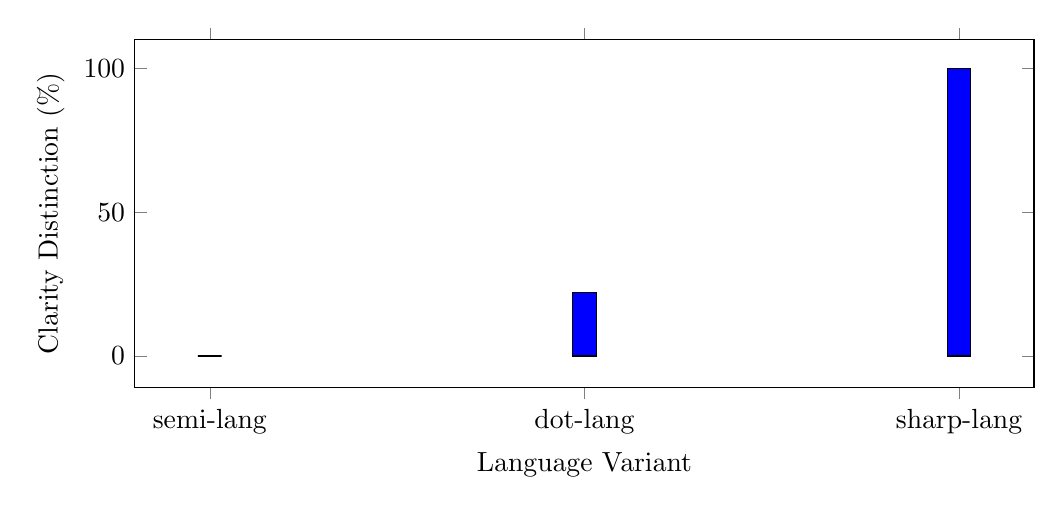
\begin{tikzpicture}
\begin{axis}[
    xlabel={Language Variant},
    ylabel={Clarity Distinction (\%)},
    ymax=110,
    width=13cm,
    height=6cm,
    xtick={1,2,3},
    xticklabels={semi-lang, dot-lang, sharp-lang},
    ybar,
    bar width=0.3cm,
]
\addplot[fill=blue] coordinates {(1,0) (2,22) (3,100)};
\end{axis}
\end{tikzpicture}

\caption{Summary of the experiment results for the second code snippet using the Gemma 3 12B model with the modified prompt.}
\label{fig:result-summary-another}
\end{figure}



GPT 5.2 Instant performed pretty much the same as before the prompt modification,
because it was already producing correct fixes all the time, not falling back to
C-like syntax for obfuscated language variants,
showing no distinction in clarity for any language variant.
That is, GPT 5.2 Instant was already exhibiting the modified instructions even
before the prompt modification. Thus, no behavioral change was observed
with GPT 5.2 Instant after the prompt modification.

\begin{figure}[htbp]
\begin{lstlisting}
Fix the syntax error in the code below using ONLY the error message,
without using the pre-trained knowledge.

Error message:
{{syntax error message here}}

Code:
```
{{code snippet with syntax error here}}
```

Output only the fixed code inside the triple backquote code block.
Note the syntax of the code above may be DIFFERENT from C-like languages.
So do not fix the code assuming it is a C-like language, unless you are
very sure, from the error message and the code above, it is actually
a C-like syntax. Make MINIMAL CHANGES to the code to fix the syntax error
and make it a TOP PRIORITY to use the information from the error message.
FIRST try to fix the error only using symbols that either directly appear
or suggested in the error message.
VERY IMPORTANT: DO NOT USE symbols from C-like syntax to fix the syntax error
unless it is suggested by the error message, or you have high confidence that
the syntax of the code is definitively C-like.
\end{lstlisting}
\caption{Prompt template with additional instructions at the end
to make the LLM judge not rely too much on its pre-trained knowledge
when producing fixes for obfuscated code snippets.}
\label{fig:prompt-template-2}
\end{figure}



% \begin{itemize}
% \item
% 50/50 correct fixes for \emph{dot-lang} with the worst error message
% \item
% 50/50 correct fixes for \emph{dot-lang} with the informative error message
% \item
% 50/50 correct fixes for \emph{dot-lang} with the worst error message
% \item
% 50/50 correct fixes for \emph{dot-lang} with the informative error message
% \item
% 45/50 correct fixes for \emph{sharp-lang} with the worst error message
% \item
% 50/50 \emph{sharp-lang} with the informative error message
% \end{itemize}

\section{Discussion on the Observed Behavior of LLM Models}
We first speculate on probable explanations of the different observed behaviors of
LLM model variants in our experiment, and then discuss the implications of
our results for future LLM-as-a-judge approach parser error message clarity.

\subsection{On the Observed Behaviors of LLM Models}
Before the detailed discussion, it should be clarified that
these are not definitive analysis of the observed behaviors,
but rather speculation for probable explanations for our results.
LLMs are often described as black boxes due to the difficulty in interpreting
their internal workings. Therefore, it is challenging to definitively pinpoint
the exact reasons behind their behavior, especially when proving a concept of
an idea for a new method rather than conducting an extensive survey across
various models and settings for an established method.

\subsubsection{Why 12B variant of Gemma 3 model performed better than others?}
Our speculations on why only the mid-sized 12B variant performed well
in our experiment is that it happens to strike a good balance between
model capacity and granularity of prior-knowledge.
We think that the smaller 4B variant may not have sufficient capacity
to effectively reason about probable fixes according to the information
provided by the error message for a less common language syntax, using
square brackets instead of curly braces. This did not surprise us,
as smaller models tend to struggle with complex reasoning tasks.
On the other hand, we did not expect at first the larger 27B variant
would fail to perform well, as larger models are generally expected
to perform better in benchmarks of various tasks.

Figure \ref{fig:results-summary} illustrates that 12B variant of Gemma 3
outperformed much larger and sophisticated GPT-5.2 model variants.
Because of the flexibility and advanced reasoning capability of GPT-5.2 models,
they could think of various other possible causes of syntax errors
beyond the prior knowledge of C-like syntax, sometimes considering less
often used programming languages. One can observe this from their
triple backquoted outputs, which sometimes specify a programming language
after the opening triple backquote (e.g., \verb|```python|), for both
\emph{bracket-lang} and \emph{gibberish-lang} variants.
This has negative effects from both sides on the clarity distinction metric.
It raises the baseline performance for the worst error message
because it sometimes leads to correct fixes without any useful information.
It also lowers the performance for the informative error message because
it sometimes leads to incorrect fixes, considering wide range of 
possible fixes, instead of focusing on the most probable fix suggested
by the informative error message.
In contrast, the outputs from Gemma 3 12B model specified
no programming language at all after the opening triple backquote
for \emph{bracket-lang} and only a few times for \emph{gibberish-lang}. 


\subsubsection{Why the larger GPT-5.2 model did not perform better?}
GPT-5.2 model variants did not perform as well as the Gemma 3 12B model
for the \emph{bracket-lang} and \emph{gibberish-lang} variants
in terms of clarity distinction metric.
There seems to be two aspects playing a role here.
First, the baseline performance of GPT 5.2 model variants are higher,
that is more number of correct fixes with the worst error message,
compared to Gemma 3 model variants, which could fix none among 50 trials
in the \emph{bracket-lang} and \emph{gibberish-lang} language variants.
Because of the flexibility and advanced reasoning capability of GPT-5.2 models,
they could think of various other possible causes of syntax errors
beyond the prior knowledge of C-like syntax, sometimes considering less
often used programming languages. This sometimes led to correct fixes
even with the worst error message without any useful information.
Secondly, it seems that the larger and more sophisticated models are likely
to have stronger prior-knowledge influence on existing programming languages,
In particular for the \emph{gibberish-lang} variant, it produces unintended wrong
fixes when it uses the knowledge about how the symbols \verb|@| and \verb|#| are
used in existing programming languages. For example, it sometimes interprets
\verb|#| as a start of a comment line, leading to incorrect fixes.
Such intermediate step of "thinking" is in fact observable
when using GPT-5.2 Thinking model through the ChatGPT website.

We suspect the reason for this is that the larger and sophisticated models
are able to explore more possibilities for fixing syntax errors.

\subsubsection{Why code-specialized CodeGemma model variants did not perform well?}
One interesting aspect in our result is that the specialized models
tuned for coding tasks, CodeGemma model variants, did not perform well
in our experiments. We could think of two possible reasons for this.

One possible reason is that such models are more heavily biased towards
existing programming language syntax and compiler implementations,
which makes it difficult to mitigate the prior-knowledge dominance problem.
The goal of coding-specialized models is to perform well on
existing programming languages, and fine-tuned to perform well
exactly at such tasks. As a result, they may be tuned to lean further over
prior knowledge on programming language syntax, when performing tasks.
So they are likely to be less flexible to deal with newly invented
programming language syntax, especially with obfuscated inputs.

Another possible reason is simply because of limited model size for quick response.
Such lightweight coding-specialized models typically have smaller parameter size
compared to general-purpose LLM models, in order to scan the codebase and
make a quick response. This may limit their capability to perform the task of
fixing syntax errors in obfuscated code snippets. Our experimental result that
8B parameters of Gemma 3 model variant, which is close to 7B parameters of
CodeGemma model variants, did not perform well either, supports
this possibility.

In future work, it would be interesting to explore more coding-specialized models,
either with larger parameter counts or whose unspecialized variants of similar size
already exhibit distinguishing behavior for the error messages of obfuscated inputs.
This would help clarify whether the observed inability to distinguish
error messages for obfuscated inputs is a general phenomenon across
coding-specialized models. If so, further exploration may clarify whether
coding specialization or model size is the more dominant factor
for the observed behavior.

\subsubsection{Why was the second code snippet more challenging?}
To our intuition, a missing delimiter is a simpler case of syntax error,
which is trivial to understand and fix, compared to the syntax error
in the first code snippet involving mismatched pair of delimiters. 
We speculate that its `triviality' may have contributed to the difficulty
in mitigating the prior-knowledge dominance problem.

There is only one terminal symbol in the second code snippet
related to the syntax error, which is the delimiter itself.
Obfuscating only that single terminal symbol makes less difference
to existing programming language syntax, compared to obfuscating
a pair of terminal symbols, as in the first code snippet.
We conjecture that this may make it easier for the LLM judge to fall back to
its prior knowledge of existing programming languages,
when it is one symbol different from the original syntax,
compared to when it is two symbols different. This is a probable
explanation for the 12B variant of Gemma 3 model making more
incorrect fixes for obfuscated inputs with informative error messages,
even when informative error messages are provided.

In Figure \ref{fig:result-summary-another}, we can observe that
the clarity distinction for \emph{dot-lang} variant is much lower
than that for \emph{sharp-lang} variant, which is consistent
with the speculation above involving number of difference in obfuscated symbols,
as dot (\verb|.|) is more commonly used as a delimiter
in existing programming languages than sharp (\verb|#|).
Therefore, even after mitigating the prior-knowledge dominance
with additional instructions in the prompt template,
\emph{dot-lang} may have felt somewhat more similar to existing
programming language syntax than the \emph{sharp-lang} variant,
leading to more incorrect fixes relying on prior knowledge of
existing programming languages for the Gemma 3 12B model.

The behavior of GPT 5.2 Instant model variant was completely different.
Unlike the Gemma 3 12B model, GPT 5.2 Instant was able to produce correct fixes for
all the time for all language variants, including the original and the obfuscated ones,
regardless of error message quality. This indicates that GPT 5.2 Instant was able to
fix syntax errors independent of the prior knowledge of which symbols are
more commonly used as delimiters in existing programming languages.
It is not impossible to interpret this seemingly opposite behavior also
due to `triviality' of the syntax error. One possible explanation for this behavior
is that GPT 5.2 has sufficient capability to structurally reason about comparatively
simpler delimiter-missing syntax errors, agnostic to the choice of terminal symbols,
that is, whether it is semicolon, dot, or sharp. This is of course a wild guess,
but one could imagine that GPT-5.2 model may have internalized
the structural concept of `delimiter', independent of actual delimiter symbol,
but somehow not for a pair of symbols used as parenthesis-like matching structure.

\section{Related Work on Prior-Knowledge Bias in LLMs}
Prior-knowledge bias in LLMs has been addressed along three complementary directions.
First, prompt-side mitigation such as self-debiasing adds explicit
negative continuations to steer generations away from biased priors
\cite{schick2021selfdebias}.
Second, calibration methods like contextualized logit adjustment reduce bias
from spurious priors in few-shot settings by normalizing scores across prompts
\cite{zhao2021calibrate}.
Third, model-editing techniques such as ROME surgically override internal
factual associations to prevent dominant prior knowledge from overwhelming
new evidence \cite{meng2022rome}.
Our use of obfuscation and prompt instructions is aligned with
the first two categories -- reducing reliance on memorized syntax so that
the provided error message becomes the primary signal.
The last direction of model-editing work suggests a complementary path
if parser-facing LLM judges must operate without input obfuscation.

% TODO re confirm and revise may be needed
Beyond prior-knowledge mitigation, recent studies have examined the reliability and robustness of LLM-as-a-judge methodologies across domains. Anghel et al. diagnose bias and instability in LLM evaluators and propose a scalable pairwise meta-evaluator \cite{anghel2025diagnosing}. Vasilev et al. validate LLM-as-a-judge workflows for medical text summarization \cite{vasilev2026llmasjudge}, while Keith analyzes coherence judgments made by LLMs \cite{keith2025llmjudge}. Zhang et al. introduce multi-model judgment frameworks for safety-centered evaluation without ground truth \cite{zhang2026multimodel}. Anghel et al. also present rubric-guided procedures to improve transparency and consistency in LLM evaluation \cite{anghel2025courseevalai}. Complementary compiler-front-end work such as BoostPolyGlot highlights diagnostic behaviors under fuzz testing \cite{liu2025boostpolyglot}, motivating our emphasis on obfuscation and prompt-control when assessing parser error-message clarity with LLMs.

\section{Conclusion and Future Work}
Our work demonstrates that 
LLM-as-a-judge approach could be used to evaluate clarity of parser error messages,
provided that the prior-knowledge dominance problem is mitigated
through obfuscation of input code snippets. However, not all LLM models
are capable of such evaluation, as only some of the model variants we tried
exhibited the desired behavior in our experiment.

Our result suggests that larger model size does not necessarily
lead to better capability to evaluate error message clarity,
as only the mid-sized 12B variant of Gemma 3 model exhibited the desired behavior,
while both smaller 8B and larger 32B variants did not.
Overly sophisticated and overly specialized models, as well as overly small models,
seem to struggle with mitigating the prior-knowledge dominance problem.
By analogy to human participants, novices may have difficulty understanding the information
provided by the error message, while extremely knowledgeable experts
do not even need to read error messages to fix syntax errors. Therefore,
our conjecture is that there may be a sweet spot in model capacity for
evaluating error message clarity.

For future work, it would be interesting to explore more LLM model variants,
to clarify what model characteristics are important for evaluating
error message clarity. It would also be interesting to explore more diverse
code snippets with different types of syntax errors, to see how generalizable
our approach is.

Next, we should compare two different informative error messages with different levels
of clarity, to see if the LLM judge can distinguish between them.
In this work, we only compared an informative error message against
the worst uninformative error message. We have been successful in distinguishing
clarity between one informative error message
against the baseline uninformative error message, as a proof of concept.
The next step would be to see if the LLM judge can distinguish
more subtle differences in clarity, by comparing two different
informative error messages from different styles of parser implementations
for the same programming language syntax.

Another important future work is to automate obfuscation and prompt design.
In this work, we manually obfuscated the code snippets and designed the prompts.
Even in our simple code snippets different obfuscation schemes affected the results
in clarity distinction metrics. Good obfuscation schemes and prompt designs
may vary depending on the code snippets and types of syntax errors.
Automating these steps would make our approach more practical
for real-world applications, where a wide variety of code snippets
and error messages need to be evaluated efficiently.
    
Overall, our work opens up new possibilities for leveraging LLMs
in the domain of programming language tooling, particularly
in enhancing the usability of parsers through better error messages.


%%%%%%%%%%%%%%%%%%%%%%%%%%%%%%%%%%%%%%%%%%
%\isPreprints{} % If the paper is ``preprints'', please uncomment this parenthesis.
%\printendnotes[custom] % Un-comment to print a list of endnotes

\reftitle{References}
\bibliography{references}
% Please provide the correct journal abbreviation (e.g. according to the “List of Title Word Abbreviations” http://www.issn.org/services/online-services/access-to-the-ltwa/).
% Citations and References in Supplementary files are permitted provided that they also appear in the reference list here. 



% If authors have biography, please use the format below
%\section*{Short Biography of Authors}
%\bio
%{\raisebox{-0.35cm}{\includegraphics[width=3.5cm,height=5.3cm,clip,keepaspectratio]{Definitions/author1.pdf}}}
%{\textbf{Firstname Lastname} Biography of first author}
%
%\bio
%{\raisebox{-0.35cm}{\includegraphics[width=3.5cm,height=5.3cm,clip,keepaspectratio]{Definitions/author2.jpg}}}
%{\textbf{Firstname Lastname} Biography of second author}

% For the MDPI journals use author-date citation, please follow the formatting guidelines on http://www.mdpi.com/authors/references
% To cite two works by the same author: \citeauthor{ref-journal-1a} (\citeyear{ref-journal-1a}, \citeyear{ref-journal-1b}). This produces: Whittaker (1967, 1975)
% To cite two works by the same author with specific pages: \citeauthor{ref-journal-3a} (\citeyear{ref-journal-3a}, p. 328; \citeyear{ref-journal-3b}, p.475). This produces: Wong (1999, p. 328; 2000, p. 475)


\PublishersNote{}
%\isPreprints{} % If the paper is ``preprints'', please uncomment this parenthesis.
\end{document}
